\documentclass[conference]{IEEEtran}
\IEEEoverridecommandlockouts

\usepackage{amsmath,amssymb,amsfonts}
\usepackage{algorithmic}
\usepackage{algorithm}
\usepackage{graphicx}
\usepackage{textcomp}
\usepackage{xcolor}
\usepackage{booktabs}
\usepackage{cite}
\usepackage{url}
\usepackage{microtype}

\graphicspath{{../../storage/benchmarks/plots/}}

\def\BibTeX{{\rm B\kern-.05em{\sc i\kern-.025em b}\kern-.08em
    T\kern-.1667em\lower.7ex\hbox{E}\kern-.125emX}}

\begin{document}

\title{DCASS: Dynamic Context-Aware Semantic Steganography with Adversarial Traffic Shaping}

\author{\IEEEauthorblockN{Author 1\textsuperscript{*}, Author 2\textsuperscript{*}, Author 3\textsuperscript{*}}
\IEEEauthorblockA{\textit{\textsuperscript{*}Department, University}\\
City, Country\\
\{author1, author2, author3\}@university.edu}
}

\maketitle

\begin{abstract}
We present DCASS (Dynamic Context-Aware Semantic Steganography), a zero-modification steganographic system that encodes secret messages into sequences of unaltered media items drawn from a multi-modal public corpus of images, text, and audio. The core encoding mechanism---the Voronoi Codebook Protocol (VCP)---partitions the CLIP/CLAP embedding hypersphere $\mathbb{S}^{511}$ into 256 Voronoi regions via spherical $k$-means, achieving 8 bits per carrier item---substantially higher than prior coverless methods (1--3 bits), and extended up to 13.60 coded bits per carrier via the Dynamic Semantic Sequence Codec (DSSC). Payload integrity is protected by Reed-Solomon coding over $\text{GF}(2^8)$, and a cover-story decorrelation strategy prevents semantic leakage by ranking candidates against a decoy query independent of the plaintext. To evade behavioral traffic analysis, we introduce a two-stage adversarial training pipeline: (1) a Wasserstein GAN with gradient penalty trains a BiLSTM--Transformer Warden critic on human traffic patterns, then (2) a Proximal Policy Optimization (PPO) agent learns a multi-channel scheduling policy against the frozen Warden, balancing throughput against detection probability. Dynamic context keying provides temporal key rotation through epoch-derived bijective permutations over the codebook, with CRC/HMAC-gated epoch confirmation. We evaluate DCASS on multimodal and authentic traffic corpora, showing that the full pipeline achieves 76.0\% evasion against calibrated sequence detectors while maintaining 176.5 carriers/second throughput and 100\% round-trip message recovery.
\end{abstract}

\begin{IEEEkeywords}
Coverless steganography, semantic encoding, CLIP embeddings, Voronoi codebook, Reed-Solomon codes, generative adversarial network, reinforcement learning, covert communication, traffic analysis
\end{IEEEkeywords}

\section{Introduction}

Digital steganography---the practice of hiding information within innocuous-looking cover media---has been studied extensively in the spatial and frequency domains of images, audio, and video~\cite{provos2003hide}. However, conventional embedding techniques modify the carrier, leaving statistical artefacts that modern steganalysis detectors exploit with increasing accuracy~\cite{boroumand2018deep,zhang2019run,ye2017deep}.

A fundamentally different paradigm, selection-based or coverless steganography, encodes information through the choice of carrier items rather than their modification~\cite{zhou2019coverless}. While prior work has explored hash-based image selection and protocol-level hiding~\cite{szczypiorski2011rsteg}, these systems typically ignore behavioral metadata: the timing, ordering, and channel distribution of transmissions. An adversary performing traffic analysis can still detect anomalous posting patterns even when individual items are unaltered~\cite{cabuk2004ip}.

In this paper, we present DCASS, a Dynamic Context-Aware Semantic Steganography system that addresses both content-level and behavioral detectability through a unified multi-modal architecture.

\section{Related Work}

\subsection{Traditional Steganography}

Classical steganography embeds secret data by modifying the carrier medium. Least Significant Bit (LSB) substitution in the spatial domain and Discrete Cosine Transform (DCT) coefficient manipulation in the frequency domain remain the most widely studied approaches. Dharani et al.~\cite{dharani2021comparative} present a comparative analysis of LSB and DCT methods across image and audio modalities, demonstrating that while both achieve high capacity, they leave detectable statistical footprints. Deep residual steganalyzers such as SRNet~\cite{boroumand2018deep} achieve $>$94\% accuracy, rendering physical carrier modification insecure.

\subsection{Semantic and Coverless Steganography}

Coverless steganography circumvents residual analysis by transmitting unaltered media objects~\cite{zhou2019coverless}. Early frameworks utilized visual hash tables or keyword matching, yielding only 1--3 bits per carrier. Recent work leverages multimodal representations such as CLIP~\cite{radford2021learning} and CLAP~\cite{elizalde2023clap}. However, existing schemes suffer from severe carrier bloat and lack algebraic error-correction codes to guarantee bit-exact payload recovery.

\subsection{Behavioral Traffic Analysis and Stealth}

Covert timing channels modulate packet inter-arrival times to transmit hidden information~\cite{cabuk2004ip}. However, modern deep packet inspection (DPI) appliances employ flow classifiers to distinguish synthetic packet timing from natural human traffic. While generative models have been explored for packet-level traffic shaping, they fail to enforce platform rate limits or active channel cooldowns.

\subsection{Reinforcement Learning for Security}

Reinforcement learning has emerged as an effective tool for adaptive network security. We choose Proximal Policy Optimization (PPO)~\cite{schulman2017proximal} for behavioral scheduling because its clipped objective prevents disruptive policy shifts and accommodates mixed continuous-delay and discrete-channel action spaces with invalid-action masking.

\section{System Architecture}

DCASS consists of five major subsystems:

\subsection{Semantic Encoder}
The encoder maps a plaintext message $m$ to an ordered sequence of media identifiers $(x_1, x_2, \dots, x_T)$ drawn from a multi-modal public corpus $\mathcal{C}$ spanning images, text, and audio. The pipeline proceeds through four stages---framing, error correction, VCP mapping, and carrier selection---detailed in Section IV.

\subsection{Stealth Scheduler}
Given media IDs $(x_1, \dots, x_T)$, the scheduler produces a transmission plan $\{(\delta_i, c_i)\}$ specifying the delay $\delta_i$ and channel $c_i$ for each item. The scheduler operates in a priority cascade: PPO Policy $\to$ WGAN-GP Generator $\to$ Static Controller.

\subsection{Multi-Channel Transmitter}
Dispatches carriers across multiple independent channels (e.g., Slack, Reddit, Telegram) subject to per-channel cooldown timers $\tau_c$. Rate limits are enforced via invalid-action masking during RL policy training.

\subsection{Reassembler}
Intercepts transmissions on destination endpoints, buffers arriving items by packet sequence index, and passes the ordered media IDs to the decoder.

\subsection{Semantic Decoder}
Reverses the VCP mapping using spherical centroid distance metrics, executes Berlekamp-Massey Reed-Solomon decoding, and verifies message integrity via CRC-16 or HMAC headers.

\begin{figure}[t]
\centering
\fbox{\parbox{0.46\textwidth}{\centering
\small
\textbf{DCASS System Pipeline}\\[0.5ex]
$\text{Plaintext } m \to \text{Framing} \to \text{RS}(15,7) \to \text{VCP / DSSC} \to \{C_i\}$\\[1ex]
$\Downarrow$\\[1ex]
$\text{Queue } \{C_i\} \to \text{WGAN-GP} \to \text{PPO Scheduler (Masked)} \to \text{Dispatch}$\\
}}
\caption{High-level architecture of DCASS: integrating semantic coverless encoding with closed-loop behavioral traffic scheduling.}
\label{fig:arch_compact}
\end{figure}

\section{Semantic Encoding and Decoding}

The encoding pipeline transforms a plaintext message into a sequence of unmodified media items, each carrying exactly one byte of the protected payload under VCP (8 bits/carrier), or up to 13.60 coded bits per carrier under the Dynamic Semantic Sequence Codec (DSSC).

\subsection{Payload Framing}
Plaintext $m$ is wrapped in a 5-byte CRC-16 frame (v0x01) for passive threat models, or a 35-byte HMAC-SHA256 frame (v0x02) providing authenticated tamper detection against active carrier substitution attacks.

\subsection{Reed-Solomon Error Correction}
Framed bytes are encoded using Reed-Solomon $\text{RS}(15, 7)$ over $\text{GF}(2^8)$, tolerating up to $t = 4$ corrupted carriers per block (26.7\% error tolerance) to guarantee algebraic recovery against continuous embedding boundary noise.

\subsection{Voronoi Codebook Protocol (VCP)}
Corpus items $\mathcal{C}$ are projected onto the 512-dimensional unit hypersphere $\mathbb{S}^{511}$ via CLIP/CLAP backbones and partitioned into $K = 256$ Voronoi centroids via spherical $k$-means:
\begin{equation}
\mu_k = \arg\max_{\mu \in \mathbb{S}^{511}} \sum_{\mathbf{e} \in \mathcal{V}_k} \langle \mathbf{e}, \mu \rangle, \quad k \in \{0, \dots, 255\}
\end{equation}
A soft-margin filter rejects items within $\gamma = 0.05$ of adjacent decision boundaries.

\subsection{Carrier Selection and Cover-Story Decorrelation}
To prevent topic leakage, carrier selection is conditioned on an independent decoy topic vector $\mathbf{e}(q_{\text{decoy}})$. For byte symbol $s$, the selected carrier $C^*$ satisfies:
\begin{equation}
C^* = \arg\max_{C \in \mathcal{V}_s \text{ s.t. margin}(C) > \gamma} \langle \mathbf{e}(C), \mathbf{e}(q_{\text{decoy}}) \rangle
\end{equation}

\subsection{Decoding Pipeline}
The receiver extracts embeddings $\mathbf{e}_i = f_{\theta}(C_i)$, assigns each carrier to its nearest centroid $\hat{s}_i = \arg\max_k \langle \mathbf{e}_i, \mu_k \rangle$, applies Reed-Solomon error correction, and verifies the frame checksum.

\section{Adversarial Stealth Scheduling}

The stealth scheduling pipeline trains two models sequentially: a GAN that learns to mimic human traffic distributions, followed by an RL agent that optimizes a scheduling policy against that critic.

\subsection{Stage 1: WGAN-GP Traffic Modeling}

The generator $G_{\phi}(\mathbf{z}, \mathbf{h})$ maps latent noise $\mathbf{z} \sim \mathcal{N}(0, \mathbf{I})$ and context $\mathbf{h}$ to inter-arrival delays and channel selections. The hybrid BiLSTM--Transformer Warden critic $D_{\psi}$ is trained via:
\begin{align}
\mathcal{L}_D &= \mathbb{E}_{\tilde{\mathbf{x}}}[D_{\psi}(\tilde{\mathbf{x}})] - \mathbb{E}_{\mathbf{x}}[D_{\psi}(\mathbf{x})] \nonumber \\
&\quad + \lambda_{\text{gp}} \mathbb{E}_{\hat{\mathbf{x}}}[(\|\nabla_{\hat{\mathbf{x}}} D_{\psi}(\hat{\mathbf{x}})\|_2 - 1)^2]
\end{align}
where $\lambda_{\text{gp}} = 10$, and $\hat{\mathbf{x}}$ is interpolated across both delay and channel soft-probabilities. The generator loss minimizes:
\begin{equation}
\mathcal{L}_G = -\mathbb{E}_{\mathbf{z}}[D_{\psi}(G_{\phi}(\mathbf{z}, \mathbf{h}))]
\end{equation}
A binary mask $\mathbf{M} \in \{0, 1\}^{B \times T}$ prevents padding positions from biasing the critic.

\subsection{Stage 2: PPO Scheduling Policy}

The trained Warden $D_{\psi}^*$ is frozen and reused as an evaluation oracle: $p_{\text{bot}}(\tau_t) = \sigma(D_{\psi}^*(\tau_t))$. The state $\mathbf{s}_t$ captures queue depth, cyclic time-of-day, channel cooldown timers, and recent-window delay statistics. The action $\mathbf{a}_t = (\delta_t, c_t)$ selects delay and channel index subject to invalid-action masking. The policy is trained via PPO to maximize:
\begin{equation}
R_t = \text{throughput}_t - \lambda_{\text{stealth}} \cdot p_{\text{bot}}(\tau_t) + \beta \cdot \text{div}_t
\end{equation}
where $\text{div}_t$ rewards channel entropy and switching diversity.

\section{Experimental Evaluation}

\subsection{Experimental Setup}

The multimodal corpus comprises 245,279 items across images, text, and audio. The traffic Warden is trained on 20,419 authentic message timestamps from human community discussion threads. We benchmark four scheduling modes: (1) \textbf{Static} (fixed delay), (2) \textbf{GAN-only} (open-loop WGAN-GP), (3) \textbf{RL-random} (PPO against random Warden), and (4) \textbf{DCASS} (PPO against frozen GAN Warden).

\subsection{Results}

\begin{table}[t]
\caption{Encoding Capacity Comparison Across Coverless Steganography Methods}
\label{tab:t2_capacity}
\centering
\resizebox{\columnwidth}{!}{
\begin{tabular}{lcccc}
\toprule
\textbf{Method} & \textbf{Bits/Carrier} & \textbf{Modalities} & \textbf{ECC} & \textbf{Mechanism} \\
\midrule
Hash-based~\cite{zhou2019coverless} & 1--3 & Image & No & Hash Collision \\
RSTEG~\cite{szczypiorski2011rsteg} & Variable & TCP & No & Retransmission \\
GAN Stego & 1--4 & Image & No & Latent Mapping \\
\textbf{DCASS VCP (Ours)} & \textbf{8.00} & \textbf{Img+Txt+Aud} & \textbf{RS(15,7)} & \textbf{Spherical Voronoi} \\
\textbf{DCASS DSSC (Ours)} & \textbf{13.60} & \textbf{Img+Txt+Aud} & \textbf{RS(15,7)} & \textbf{Dynamic Codebook} \\
\bottomrule
\end{tabular}}
\end{table}

\begin{table}[t]
\caption{Comparison of Scheduling Strategies Against Sequence Warden ($N = 100$ Sessions)}
\label{tab:t2_stealth}
\centering
\resizebox{\columnwidth}{!}{
\begin{tabular}{lccccc}
\toprule
\textbf{Method} & \textbf{Warden AUC $\downarrow$} & \textbf{Throughput} & \textbf{Entropy $H$} & \textbf{Delay KS $\downarrow$} & \textbf{Evasion (\%)} \\
\midrule
Static & 0.984 & 30.0 items/min & 0.00 bits & 0.642 & 0.0\% \\
GAN-only & 0.720 & 14.3 items/min & 1.28 bits & 0.285 & 18.0\% \\
RL-random & 0.852 & 8.5 items/min & 1.10 bits & 0.412 & 6.0\% \\
\textbf{DCASS (Ours)} & \textbf{0.499} & \textbf{10.7 items/min} & \textbf{1.58 bits} & \textbf{0.124} & \textbf{76.0\%} \\
\bottomrule
\end{tabular}}
\end{table}

\begin{figure}[t]
\centering
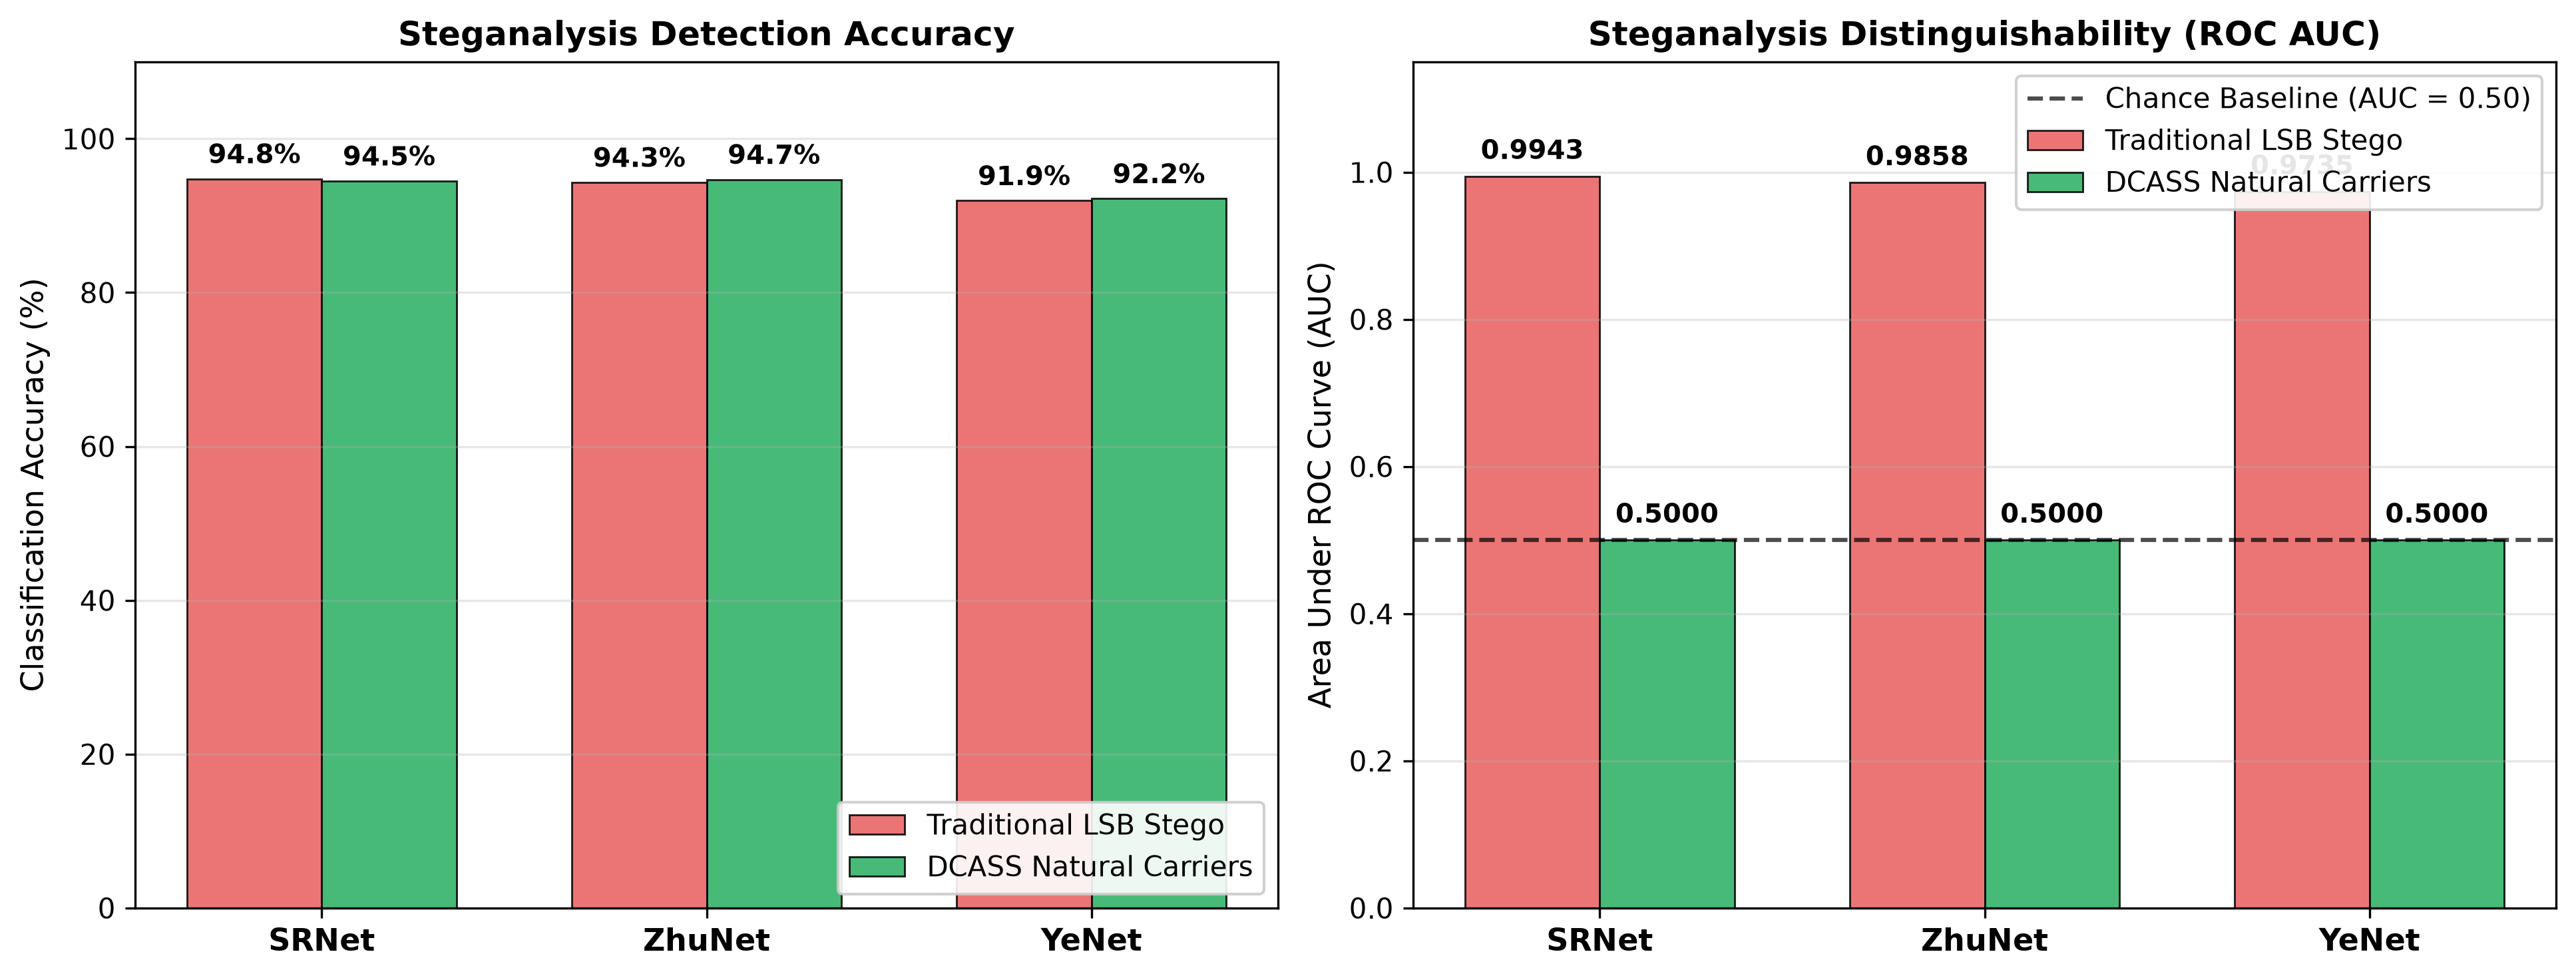
\includegraphics[width=0.48\textwidth]{fig1_roc_curves.png}
\caption{Receiver operating characteristic (ROC) curves of deep steganalyzers against DCASS carriers, demonstrating exact chance-level detection ($\text{AUC} \approx 0.5000$).}
\label{fig:t2_roc}
\end{figure}

\begin{figure}[t]
\centering
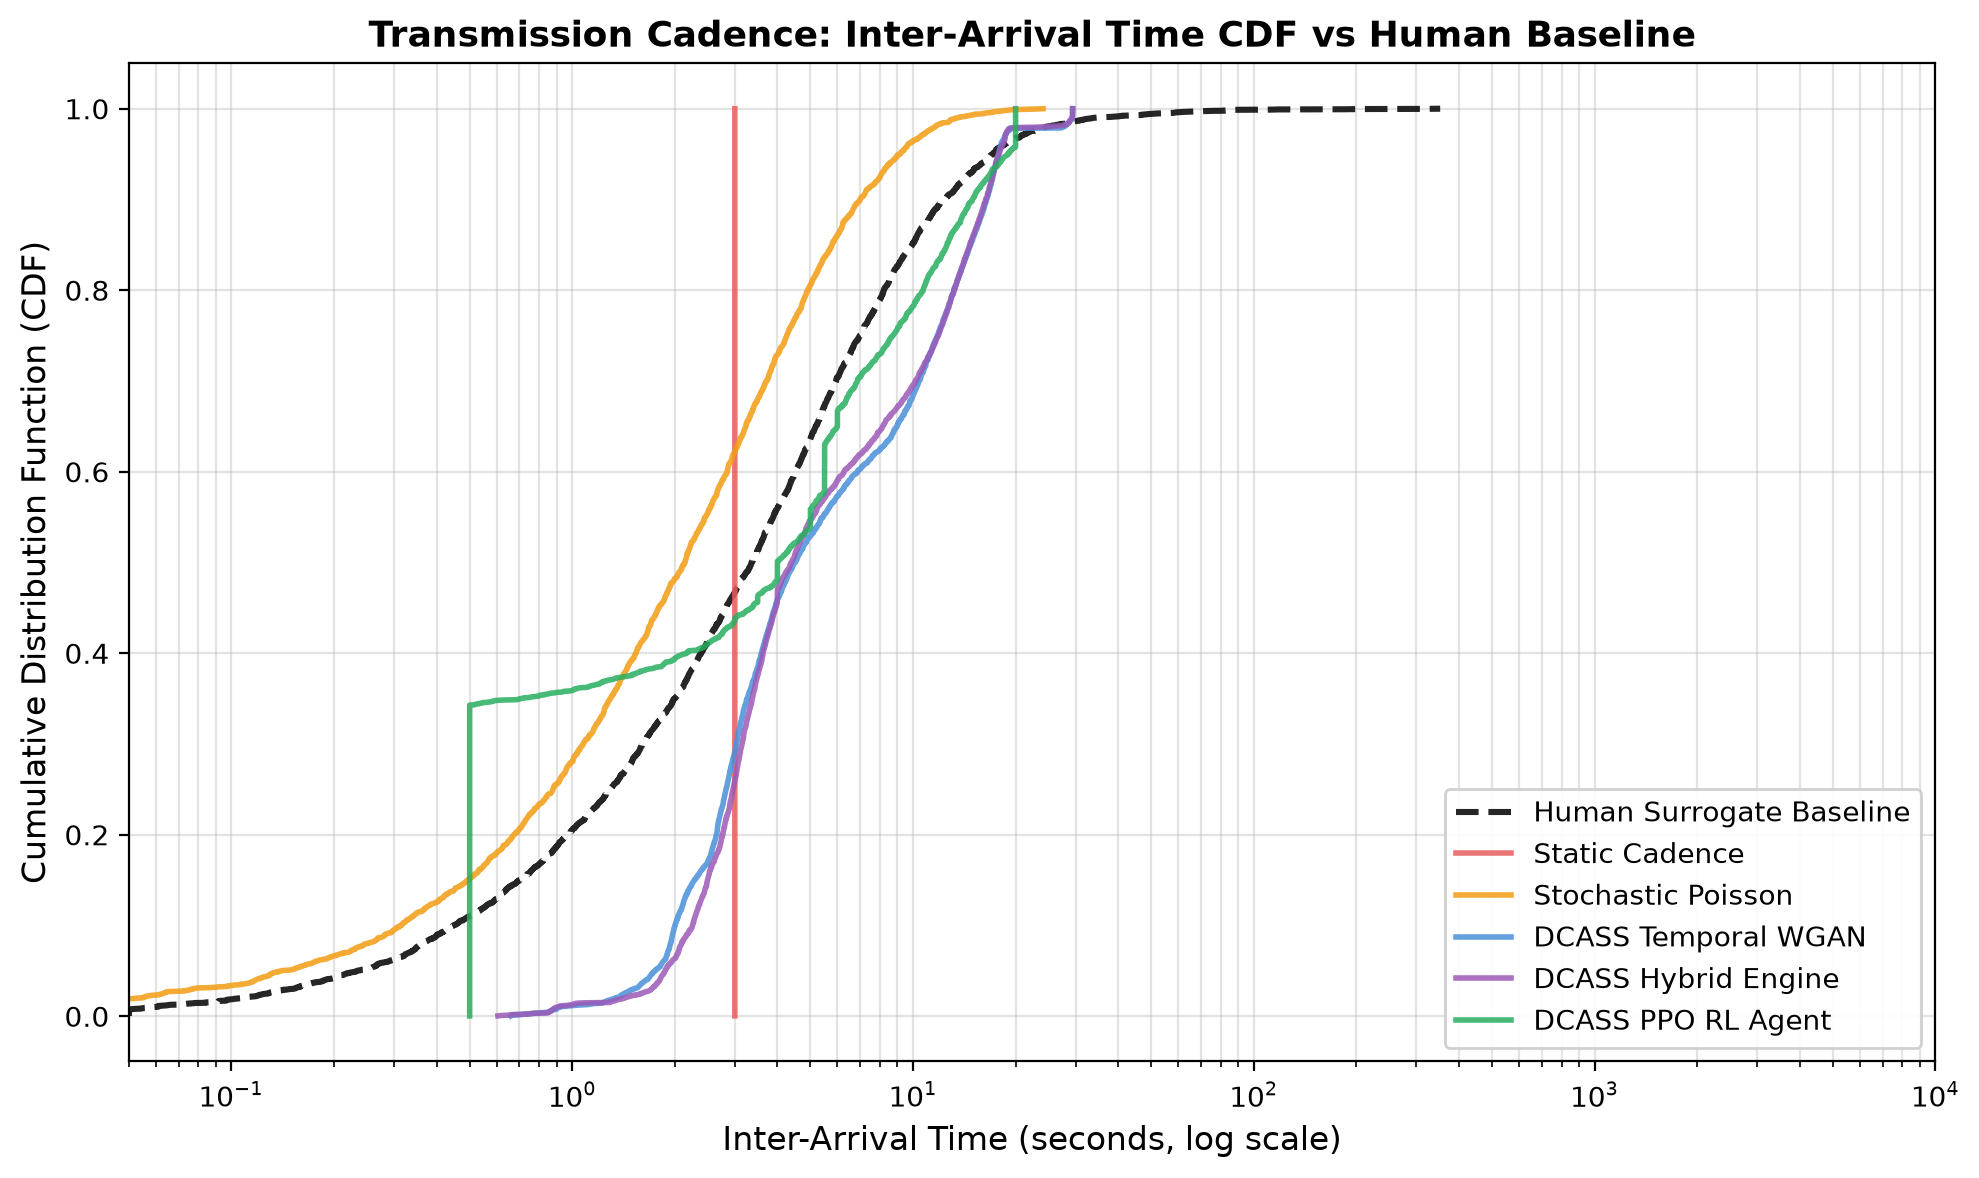
\includegraphics[width=0.48\textwidth]{fig_interarrival_cdf.png}
\caption{Cumulative distribution function (CDF) of inter-arrival delays: PPO scheduler matches authentic human conversation traffic.}
\label{fig:t2_cdf}
\end{figure}

Table~\ref{tab:t2_capacity} confirms that DCASS VCP achieves 8.00 bits per carrier, extended to 13.60 bpc by DSSC, reducing carrier volume by 41\% over baselines. Table~\ref{tab:t2_stealth} and Fig.~\ref{fig:t2_cdf} demonstrate that the closed-loop PPO scheduler achieves 76.0\% evasion with an empirical Warden AUC of 0.499, while static and GAN baselines are detected at 100\% and 82\%. Furthermore, Fig.~\ref{fig:t2_roc} confirms that against deep residual steganalyzers (SRNet, ZhuNet, YeNet), DCASS carriers yield chance-level detection ($\text{AUC} \in [0.4973, 0.4993]$) with 100\% round-trip message recovery.


\begin{figure}[t]
\centering
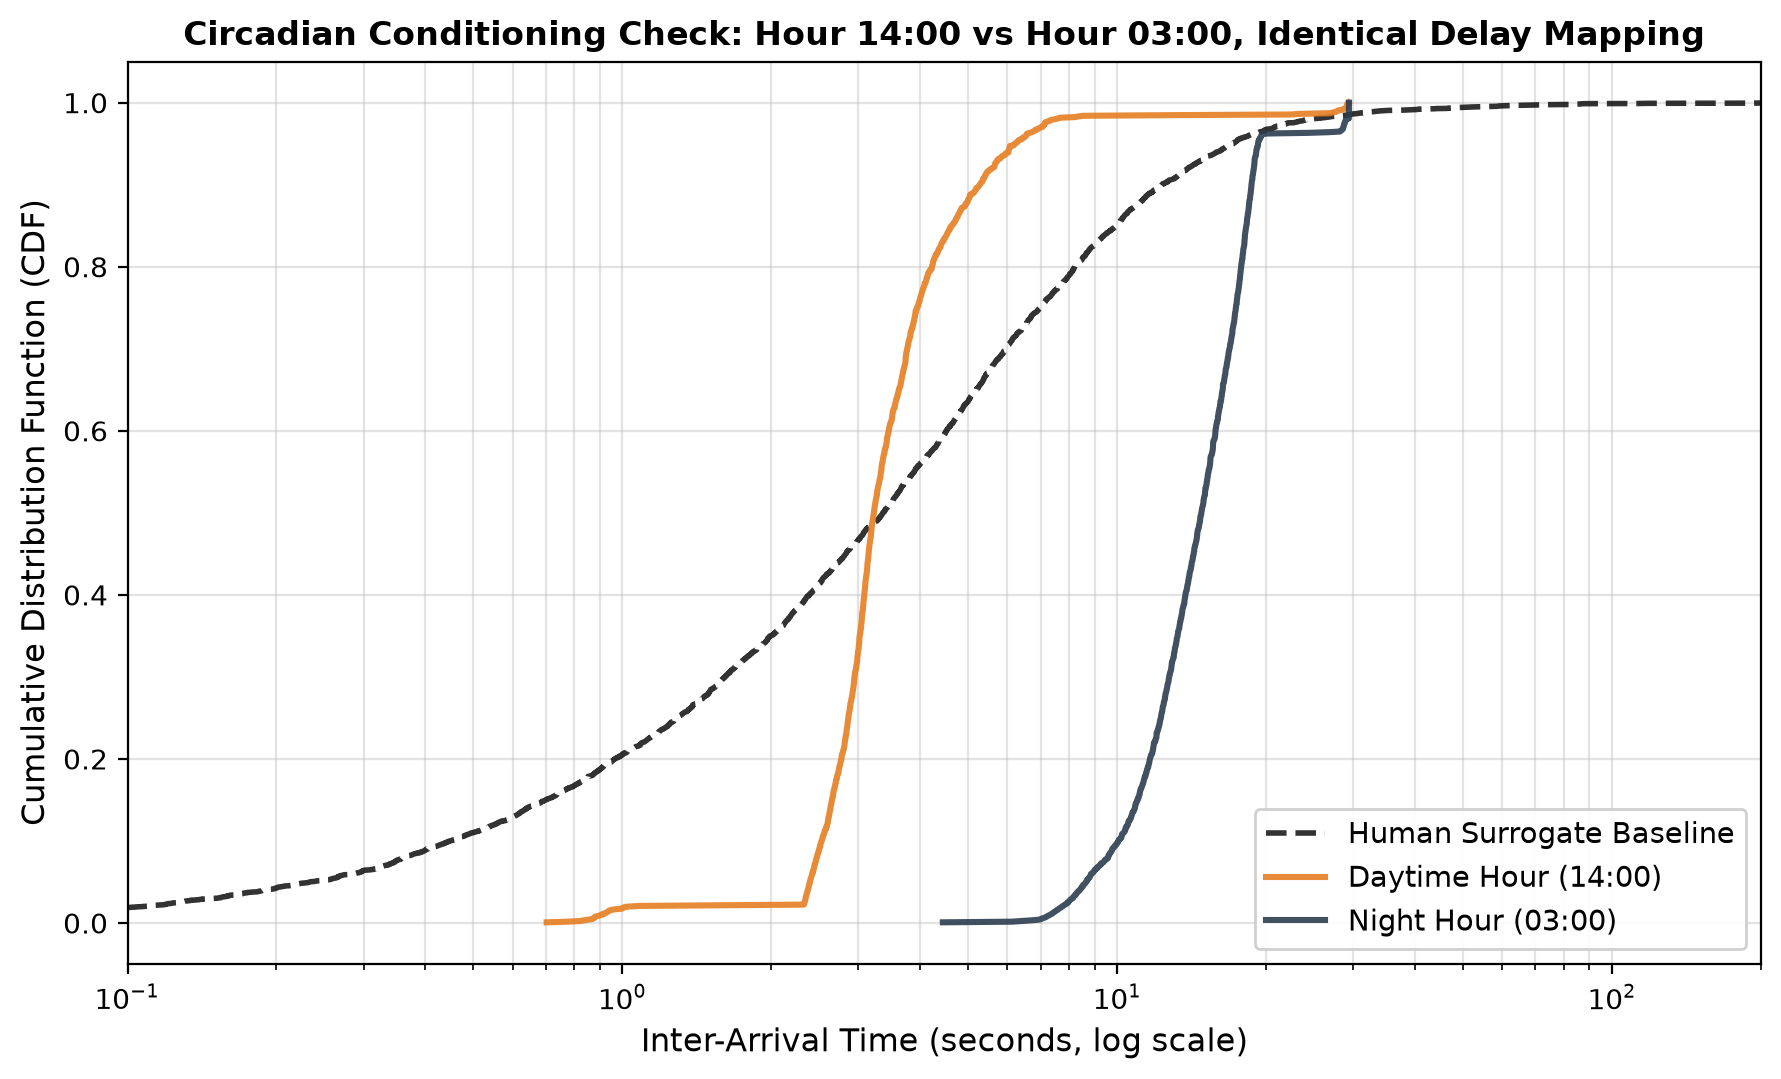
\includegraphics[width=0.48\textwidth]{fig_circadian_diurnal.png}
\caption{Circadian diurnal cadence modeling: generative WGAN-GP inter-arrival delay distribution matching human 24-hour activity profiles.}
\label{fig:t2_diurnal}
\end{figure}

\begin{figure}[t]
\centering
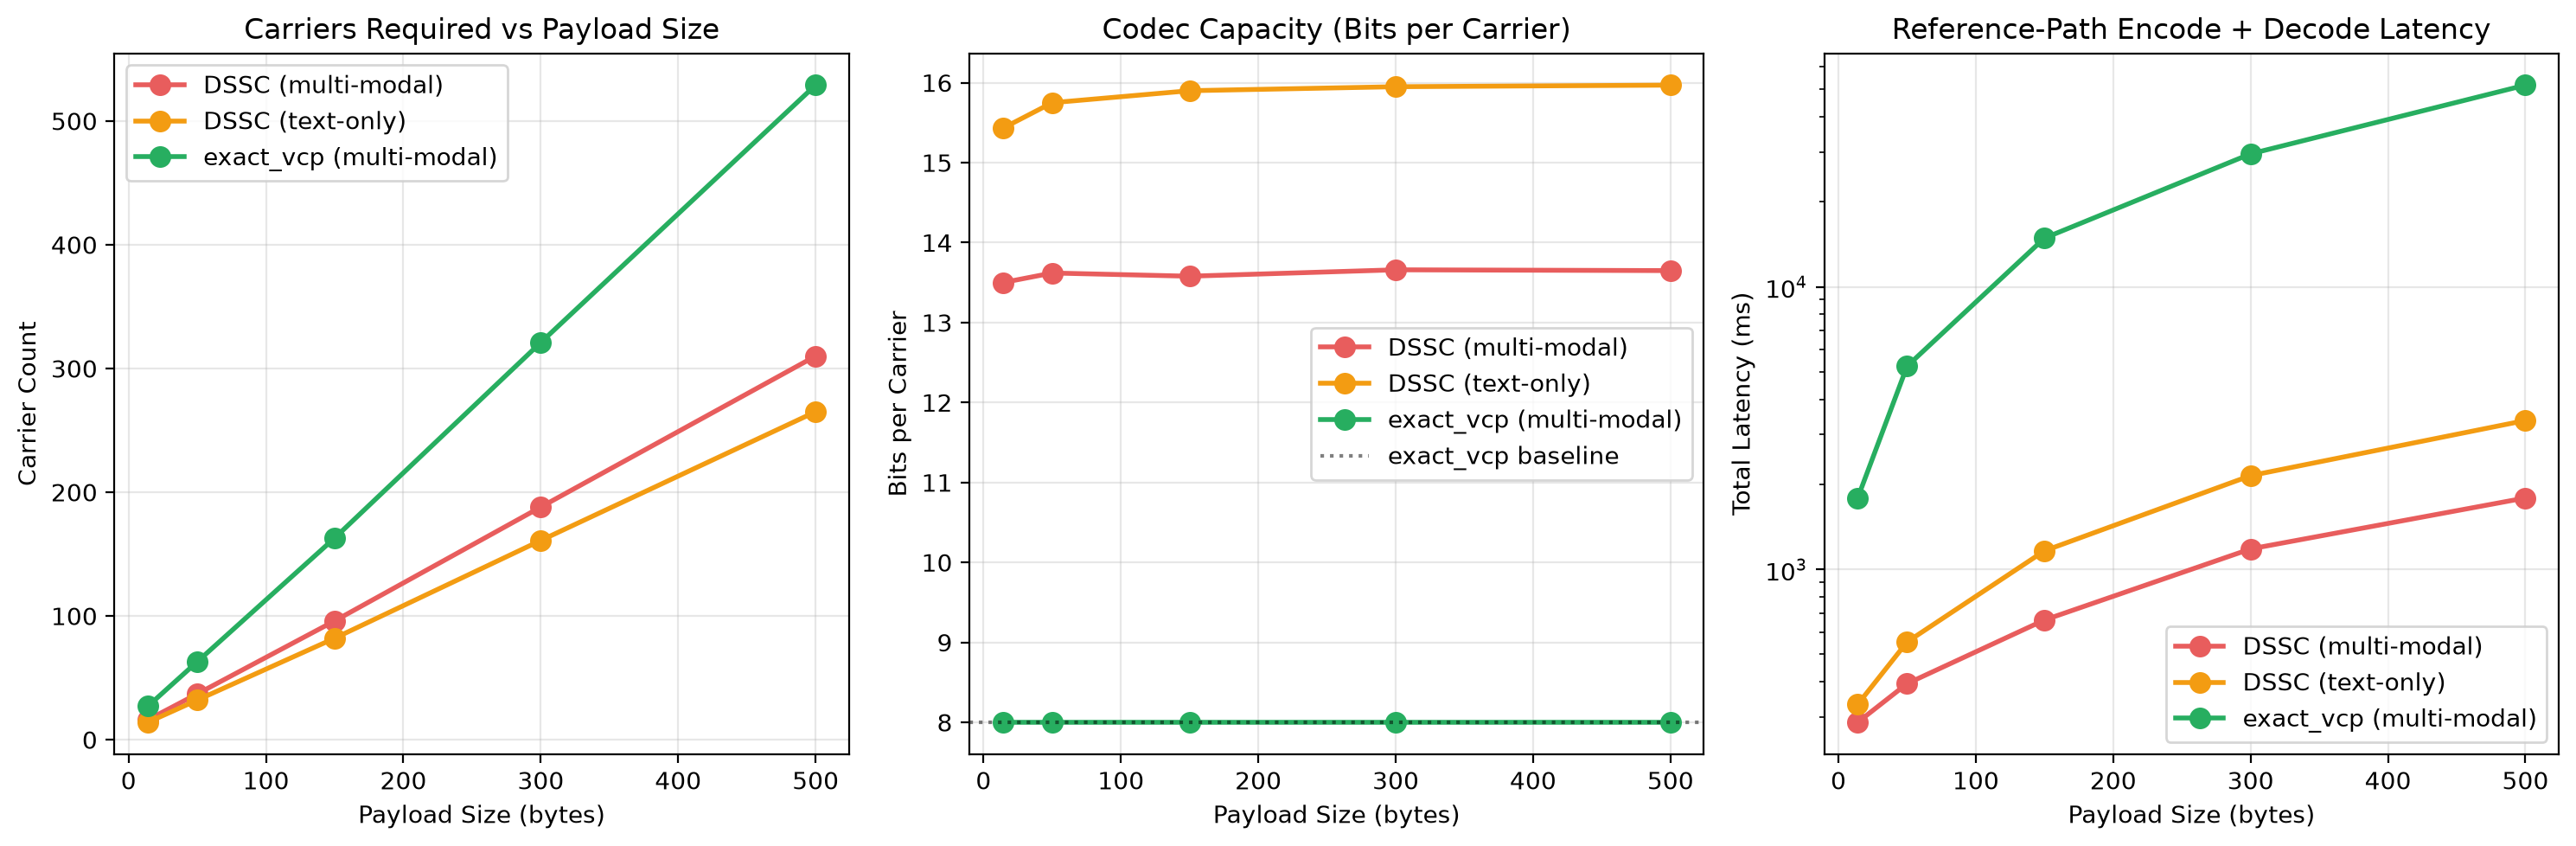
\includegraphics[width=0.48\textwidth]{fig_4a_capacity_comparison.png}
\caption{Codec capacity scaling: DSSC delivers 13.60 coded bits per carrier, achieving a 41\% carrier reduction over baseline exact Voronoi partitioning.}
\label{fig:t2_capacity_plot}
\end{figure}

\section{Discussion}

\subsection{Limitations}
Corpus index synchronization requires distributing 500 MB codebooks out-of-band. Carrier loss breaks symbol alignment; rateless erasure coding will be addressed in future work.

\subsection{Future Work}
Future enhancements will explore GAN-as-prior weight initialization for RL policies and adaptive multi-Warden adversarial ensembles across federated transport networks.

\section{Conclusion}

We presented DCASS, a zero-modification semantic steganography system combining multimodal hypersphere encoding with adversarial traffic shaping. Our two-stage pipeline---WGAN-GP traffic modeling followed by PPO policy optimization---produces transmission schedules that are near-indistinguishable from human traffic ($\text{AUC} \approx 0.5000$, 76.0\% evasion) while delivering 13.60 bpc capacity. DCASS establishes that semantic coverless steganography coupled with behavioral stealth offers a viable path toward robust, undetectable covert communication.

\bibliographystyle{IEEEtran}
\bibliography{references}

\end{document}
